%%%%%%%%%%%%%%%%%%%%%%%%%%%%%%%%%%%%%%%%%%%%%%%%%%%%%%%%%%%%%%%%%%%%%%%
%
%   Presentation of Beamer UNL Theme
%   Beamer Presentation by Chris Bourke
%
%%%%%%%%%%%%%%%%%%%%%%%%%%%%%%%%%%%%%%%%%%%%%%%%%%%%%%%%%%%%%%%%%%%%%%%

\documentclass{beamer}

\usetheme[hideothersubsections]{UNLTheme}
\usepackage[postscript]{ucs}
\usepackage[utf8x]{inputenc}

\title{Performance Modeling and
Design of Computer Systems- Ch 2 \\
Queueing Theory Terminology}
\author{Debobroto Das Robin} %
\institute{Kent State University}
\date{Spring 2020}




\begin{document}

%{% open a Local TeX Group
%\setbeamertemplate{sidebar}{}
\begin{frame}
        \titlepage
        \begin{center}
    \href{mailto:drobin@kent.edu}{\color{blue}{\texttt{drobin@kent.edu}}}
        \end{center}
\end{frame}

\begin{frame}
\frametitle{Overview} % Table of contents slide, comment this block out to remove it
\tableofcontents % Throughout your presentation, if you choose to use \section{} and \subsection{} commands, these will automatically be printed on this slide as an overview of your presentation
\end{frame}

\section{Queueing theory Terminology}

\begin{frame}
    \frametitle{Queueing theory Terminology-1}
    \framesubtitle{\textbf{\textit{}}}
	\begin{itemize}
		\item \textbf{Service Order}:  order in which jobs will be served by 				the server.Assume First-Come-First-Served (FCFS) if not explicitly 				mentioned
		\item \textbf{Average Arrival rate} $\lambda$, at which jobs arrive to 					the server. Ex.  $\lambda$ = 3 jobs/sec).
		\item \textbf{Mean Interarrival Time} Avg time between successive job 				arrivals. (e.g., $1/\lambda = 1/3$  sec).
		\item \textbf{Service Requirement} Time it would take the job to run on 		this server if there were no other jobs around (no queueing). Random 				Variable $S$
		
		\item \textbf{Mean Service Time($E(S)$)} This is the expected value of 				S , namely the average time required to service a job on this CPU, 						where “service” does not include queueing time. 

		\item \textbf{Average Service Rate}$\mu$, at which jobs are served. 
				$\mu = 1/{E[S]}$ 					
				  
	\end{itemize}	    
    
\end{frame}

\begin{frame}
    \frametitle{Queueing theory Terminology-2}
    \framesubtitle{\textbf{\textit{}}}
	\begin{itemize}
		\item 	\textbf{Response Time, Turnaround Time, Time in System, or 					Sojourn Time $( T )$ }: a job’s response time by 
			$T = t_{depart} - {t}_{arrive}$
		\item \textbf{Waiting Time or Delay $(T_Q )$}: time that the job spends in the queue, not being served. It is also called the “time in queue” or the \textbf{“wasted time.” }
		$E [T ] = E [T_Q ] + E [S]$. 
		\item Under FCFS service order, waiting time is  the time from when a job arrives to the system until it first receives service.
	\item \textbf{Number of Jobs in the System (N )}: This includes those jobs in the queue, plus the one being served (if any).
	\item \textbf{Number of Jobs in Queue $(N_Q )$}: This denotes only the number of jobs waiting (in
queue).
	  
	\end{itemize}	    
    
\end{frame}

\begin{frame}
    \frametitle{Queueing theory Terminology-3}
    \framesubtitle{\textbf{\textit{}}}
	\begin{itemize}
		\item \textbf{Device Utilization $(\rho_i )$} is the fraction of time 				device $i$ is busy. 
		\item Suppose we watch a device $  i$ for a long period of time. Let $ \tau $  denote the length of the
observation period. Let $B$ denote the total time during the observation period that the device is non-idle (busy). Then $\rho_i =  \frac{B}{\tau}$

	\item \textbf{Device Throughput $(X_i )$}: the rate of job completions at device/system $i$ (e.g., jobs/sec). 
	\item Let $C$ denote the total number of jobs completed at device $i$ during time $ \tau $ . Then $X_i = \frac{C}{\tau}$
	\item \textbf{Relation:}
$X_i = \frac{C}{\tau} = \frac{C}{B} * \frac{B}{\tau} = \frac{1}{\frac{B}{C}} * \frac{B}{\tau} = \frac{1}{E[S]} * \rho_i = \mu_i * \rho_i  $
	  
	\end{itemize}	    
    
\end{frame}


\section{Classification of Queueing Networks}



\begin{frame}
    \frametitle{Classfication of Queueing Networks}
    \framesubtitle{\textbf{\textit{Open Networks}}}
	\begin{itemize}
		\item open queueing network has external arrivals and departures
		\item Example
			\begin{itemize}
			\item CPU uses a time-sharing scheduler to serve a queue of jobs waiting for CPU time
			\item Router in a network serves a queue of packets waiting to be routed.
			\end{itemize}
		  
	\end{itemize}	    
    
\end{frame}

\begin{frame}
    \frametitle{Open Networks: Example}
    \framesubtitle{\textbf{\textit{Network of Queues with Probabilistic Routing}}}
	\begin{itemize}
		\item Server $i$ receives external arrivals (“outside arrivals”) with rate $r_i$ .
		\item Server i also receives internal arrivals from some of the other servers. 
		\item A packet that finishes service at server $i$ is next routed to server $j$ with 							probability $p_{ij}$ . 
		\item Multiple \textbf{“class”} of the packet, may have different probability according to 			routing scheme
		 \begin{figure}
        		\begin{center}
		            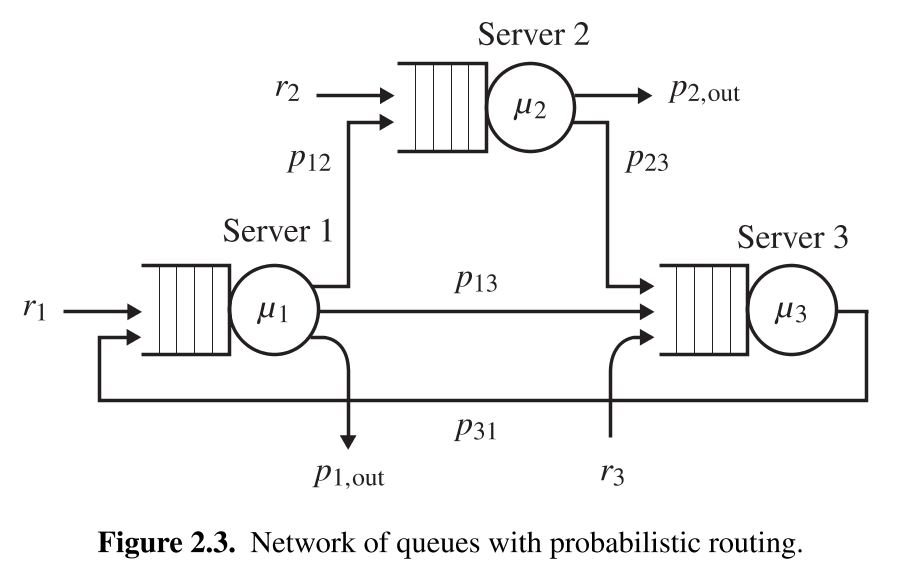
\includegraphics[scale=0.2]{images/Networkqueueswithprobabilisticrouting.jpg}
					%\caption{Sample caption.}
        		\end{center}
		    \end{figure}
		  
	\end{itemize}	    
    
\end{frame}

\begin{frame}
    \frametitle{Open Networks: Example}
    \framesubtitle{\textbf{\textit{Network of Queues with Probabilistic Routing}}}
	\begin{itemize}
			
		\item Real application in internet
			\begin{itemize}
			\item Wire delay can be  replaced by a server with some rate matching with wire delay
			\item \textbf{Goal}: is to predict RTT
			\item \textbf{Deterministic Varation}: instead of $P_{ij}$, specific path to next 						server
			\end{itemize}
			\begin{figure}
        		\begin{center}
		            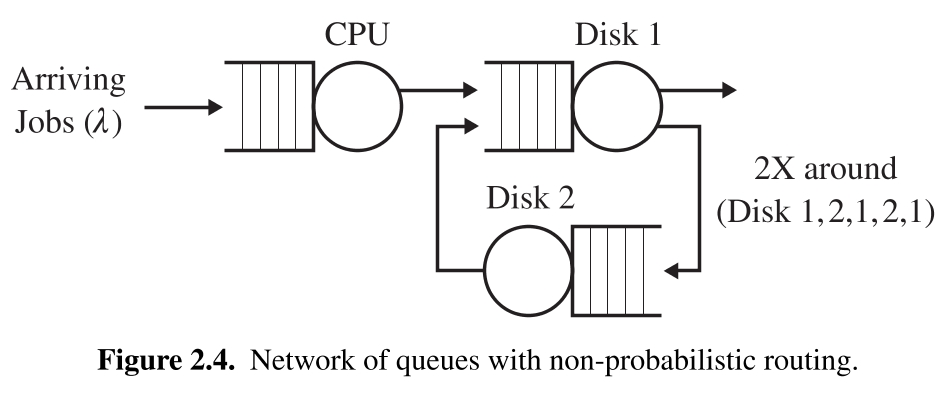
\includegraphics[scale=0.3]{images/deterministicopenqueue.jpg}
					%\caption{Sample caption.}
        		\end{center}
		    \end{figure}
		  
	\end{itemize}	    
    
\end{frame}

\begin{frame}
    \frametitle{Classfication of Queueing Networks}
    \framesubtitle{\textbf{\textit{Closed Networks-1}}}
	\begin{itemize}
		\item Closed queueing networks have no external arrivals or departures. 			They can be classified into two categories
		\item Example
			\begin{itemize}
			\item \textbf{Interactive (Terminal-Driven) Systems}
				\begin{figure}
        		\begin{center}
		            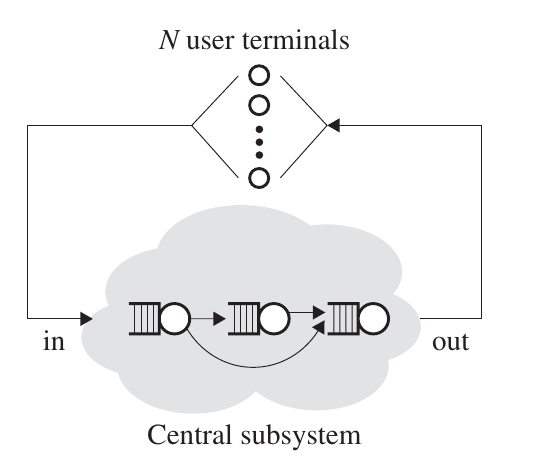
\includegraphics[scale=0.2]{images/closed_networks_1.jpeg}
					%\caption{Sample caption.}
        		\end{center}
		    \end{figure}
		    \begin{itemize}
		    \item Terminals represent users who each send a job to the “central subsystem” and then wait for a response. 
		    \item The central subsystem is a network of queues. 
		    \item A user cannot submit  next job before  previous job returns.
		    \item  Thus, the number of jobs in the system is
			fixed (equal to the number of terminals). Called the load or
				\textbf{MPL (multiprogramming level})
			\item $E [T ] = E [R] + E [Z] : E[R] =$ Avg time to get from in to out, $E[Z]$ = user thinking time 

		    \end{itemize}
		  
			\end{itemize}
		  
	\end{itemize}	    
    
\end{frame}


\begin{frame}
    \frametitle{Classfication of Queueing Networks}
    \framesubtitle{\textbf{\textit{Closed Networks-2}}}
	\begin{itemize}
		\item \textbf{Batch Systems}
			\begin{figure}
        		\begin{center}
		            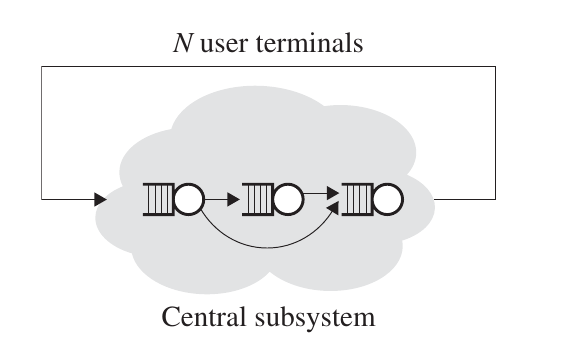
\includegraphics[scale=0.2]{images/closed_networks_2.jpeg}
					%\caption{Sample caption.}
        		\end{center}
		    \end{figure}
		    \begin{itemize}
		    \item  an interactive system with a think time of zero with dfrnt 					goal 
		    \item Goal: For a batch system, the goal is to obtain high 								throughput, so that as many jobs as possible are completed 						overnight.
		    \item \textbf{in = out} for the batch system.

		    \item  X is the number of jobs crossing “out” per second 

		    \end{itemize}
			  
	\end{itemize}	    
    
\end{frame}

\begin{frame}
    \frametitle{Classfication of Queueing Networks}
    \framesubtitle{\textbf{\textit{Open vs Closed Networks-2}}}
	\begin{itemize}
		\item Open Systems
		\begin{itemize}
			\item Throughput, X , is independent of the $\mu_i$
			\item $X$ is not affected by doubling the $\mu_i$
			\item Throughput and response time are not related.
		\end{itemize}
		\item Closed Systems
		\begin{itemize}
			\item Throughput, X , is dependent of the $\mu_i$
			\item  If we double all the $\mu_i$ holding $N$ constant, then $X$ 					changes 
			\item Higher throughput $\Longleftrightarrow$ Lower avg. response 					time
		\end{itemize}
			  
	\end{itemize}	    
    
\end{frame}

    
\end{document}